\chapter{スピン、測定、および二次元状態空間}

\lectureoverview{スピンは方向性をもつが、その成分の一つを測定すると、常に\(+1\)か\(-1\)しか返ってこない。まずこの操作上の難問を定式化し、次に非可換な測定に対して通常の集合論理がなぜ破綻するのかを見る。二次元複素ベクトル空間が適切な言語を与える。確率は振幅から導かれ、区別可能な選択肢は直交し、上--下、右--左、入--出の基底は、状態ベクトルを通常の矢印にすることなく、三つの空間方向を符号化する。}

\section{量子ビットからスピンへ}

量子ビットとして導入された二状態系を、今後は\emph{スピン}と呼ぶ。この名称の変更は空間方向を議論に持ち込むが、同時に\emph{ベクトル}という語に危険を生む。二つの異なる対象を区別しなければならない：

\begin{definition}
\emph{三次元ベクトル}は、三次元空間における通常の実ベクトルである。修飾語のない\emph{ベクトル}は、量子力学で用いられる複素状態空間のような抽象ベクトル空間の元を意味する。
\end{definition}

スピンは通常空間のある軸に対して準備することができる。しかしその状態は抽象ベクトルによって表される。これら二つの言明の関係は、我々が発見しなければならない事柄の一つであり、絵から仮定することはできない。

\section{なぜ装置を取り除けないのか}

古典力学は、系について知りながら、望むだけ小さくしか乱さない理想的な観測者を想像するよう促す。例えば、巨視的な物体を見たいとしよう。我々はそれを照らし、反射光をレンズで集め、像を増幅する。光はいくらかの力を及ぼすが、古典的な理想化では、増幅を大きくしながら強度を下げることができる。測定という考えを放棄することなく、擾乱を任意に小さくできる。

その極限操作は量子力学では失敗する。装置は改良し、遮蔽し、較正することができるが、測定を一般に、情報を与えかつ任意に非侵襲的とすることはできない。系について何かが変化する。これは、すべての測定があらゆる性質を破壊するとか、結果を再現できないという意味ではない。装置が問われている物理的問いの一部であり、測定後の状態を無視できないという意味である。

当面、装置を二つの特徴をもつ黒箱としよう。空間内で向きを変えることができ、その表示は\(+1\)か\(-1\)のいずれかを記録する。ボード上の小さな矢印は、準備されたスピンの便利なラベルである：

\begin{figure}[htbp]
\centering
\includegraphics[width=0.64\textwidth]{lecture_02_figure_02.png}
\caption{軸に沿って準備されたスピンの最初の暫定的な印。矢印は準備をラベルするものであり、まだ状態の古典的模型ではない。}
\lectureframe{00:05:15}
\end{figure}

軸を、\(z\)がボードの上向き、\(x\)が右向き、\(y\)がボードから外向きになるように選ぶ。装置が単位方向\(\hat m\)に沿って向けられているなら、その結果は
\begin{equation}
\sigma_{\hat m}=\pm1.
\end{equation}
特に、
\[
\sigma_z=\pm1,\qquad \sigma_x=\pm1,\qquad \sigma_y=\pm1.
\]
この段階では、\emph{成分}という語は操作的である。\(\sigma_z\)とは、向きを定めた装置が\(z\)に沿って向いているときに報告するものである。それはまだ、隠れた古典的矢印の\(z\)成分ではない。

\subsection{繰り返し可能性と擾乱}

\(z\)測定が\(+1\)を与えたとしよう。間に何の操作も挟まなければ、二度目の\(z\)測定も再び\(+1\)を与え、さらに繰り返しても同様である。最初の測定は、同じ問いが確定した答えをもつ状態を準備したのである。

\begin{classroomqa}
\audiencequestion{量子測定がスピンを乱すなら、なぜ直後の繰り返しは同じ結果を返すのか。}
\lecturerresponse{擾乱は無差別ではない。\(\sigma_z\)を測定することは、後の\(x\)測定や\(y\)測定で起こるはずのことを変えうるが、新たに測定された\(\sigma_z\)の値は再現可能なまま残す。有用な実験には、まさにこの限られた形の安定性が必要である。}
\end{classroomqa}

次に装置を\(180^\circ\)回転させる。上向きの向きで\(+1\)を与えたスピンは、逆向きでは\(-1\)を与える。装置を再び上向きに戻すと、結果は\(+1\)である。したがって向きが重要である。温度計は逆さまにされただけで温度の負を報告したりはしない。スピン分析器が異なる振る舞いをするのは、それが方向に関する問いを発するからである。

\begin{figure}[htbp]
\centering
\includegraphics[width=0.72\textwidth]{lecture_02_figure_03.png}
\caption{ボードは二値ラベル\(\sigma_z=\pm1\)と\(\sigma_x=\pm1\)を、\(x\)軸の手がかりとともに記録する。}
\lectureframe{00:12:46}
\end{figure}

古典的な単位ベクトルとの対比は即座に明らかである。古典的な成分は\(-1\)と\(+1\)の間を連続的に変化する。\(x\)軸に垂直な単位ベクトルは\(x\)成分がゼロである。これに対して、\(x\)に沿って向けられたスピン分析器は決してゼロを示さない。スピンが\(z\)に沿って準備された場合でも、\(+1\)または\(-1\)を示す。

\section{単一の結果とベクトル的な平均}

\(\sigma_z=+1\)を得ることによってスピンを準備し、次に\(\sigma_x\)を測定する。同一に準備された試行の半数は\(+1\)を与え、半数は\(-1\)を与える。したがって
\begin{equation}
\langle \sigma_x\rangle=0.
\end{equation}
同じ準備は次を与える
\begin{equation}
\langle \sigma_y\rangle=0.
\end{equation}
逆に、\(\sigma_x=+1\)で準備されたスピンは、その後の\(z\)または\(y\)測定の2つの結果に対して等しい確率を持つ。

その記述には二つの異なる実験が隠れている。最初の\(x\)の結果の後で\emph{同じ}スピンに対して\(\sigma_x\)を繰り返し測定しても、その結果が確認されるだけである。五十--五十の統計を得るには、同じ\(z\)状態に準備された多数のスピン、または各\(x\)測定の前にその同じ準備状態へ繰り返し戻された一つのスピンが必要である。

\begin{classroomqa}
\audiencequestion{スピンが装置に入る前に意図的に準備されていなかった場合、何が起こるか？}
\lecturerresponse{結果は依然として\(+1\)または\(-1\)であるが、その確率はスピンが実際に持つ状態に依存する。準備とは、繰り返しの試行を比較可能にする制御された手続きである。2つの測定の間に未知の操作が起こるならば、再現性はもはや保証されない。何も起こらなければ、同じ成分の結果は再現可能である。}
\end{classroomqa}

\subsection{2つの任意の方向}

\(\hat n\)に沿って向けられた分析器から\(+1\)を得ることによって、単位方向\(\hat n\)に沿ってスピンを準備する。次に別の単位方向\(\hat m\)に沿って測定する。各試行は依然として\(\pm1\)のみを与えるが、同一に準備された試行にわたる平均は
\begin{equation}
\boxed{\langle\sigma_{\hat m}\rangle=\hat n\cdot\hat m
=\cos\theta_{nm}.}
\label{eq:spin-average}
\end{equation}
黒板ではより短い記法\(\langle\sigma_m\rangle=n\cdot m\)を用いる：

\begin{figure}[htbp]
\centering
\includegraphics[width=0.74\textwidth]{lecture_02_figure_04.png}
\caption{このベクトル的な法則はアンサンブル平均に属し、個々の\(\pm1\)の結果に属するものではない。}
\lectureframe{00:23:22}
\end{figure}

式~\eqref{eq:spin-average}は以前の場合を含む。\(\hat m=\hat n\)ならば、平均は\(+1\)である。どの結果も\(+1\)を超えることはできないので、すべての試行は\(+1\)を与える。\(\hat m=-\hat n\)ならば、すべての試行は\(-1\)を与える。垂直な軸は平均ゼロと等しい頻度を与える。

\(p_+\)と\(p_-\)が2つの可能な結果の確率を表すならば、
\[
p_++p_-=1,\qquad p_+-p_-=\hat n\cdot\hat m.
\]
したがって、
\begin{equation}
p_\pm=\frac{1\pm\hat n\cdot\hat m}{2}.
\label{eq:direction-probabilities}
\end{equation}
\editorialnote{講義は2つの結果とその平均を述べている。式~\eqref{eq:direction-probabilities}はそれら2つの事実の直接的な代数的帰結である。}

\begin{classroomqa}
\audiencequestion{山括弧内の量は\emph{期待値}なのか、それとも通常の平均なのか？}
\lecturerresponse{それは多数回の繰り返しにわたる記録された結果の平均である。\emph{期待値}は標準的な用語であるが、ここでは別種の平均化を意図しているわけではない。装置は\(+1\)と\(-1\)のリストを生成し、括弧は大きなアンサンブルの極限におけるそのリストの算術平均を表す。}
\end{classroomqa}

\begin{classroomqa}
\audiencequestion{矢印\(\hat n\)は、平均法則が知られる前にすでに幾何学的な意味を持っていたのか？}
\lecturerresponse{当初それは、準備装置がどのように向けられていたかのラベルであった。反転実験と平均の\(\hat n\cdot\hat m\)への依存が、そのラベルに操作的な幾何学を与える。装置が成分の意味を定義するのであり、単一の結果が古典的な射影を与えることは決してない。}
\end{classroomqa}

これは方向の描像と離散的なデータとの最初の調和である。個々のスピンは、連続的な値の成分を持つ古典的な矢印としては振る舞っていない。それにもかかわらず、同一に準備された多数のスピンの統計は、単位3次元ベクトルの成分とまったく同じように変換する。

\section{集合としての古典的命題}

量子状態空間を構成する前に、古典系に対して論理がどのように働くかを考える。可能な状態が集合\(\Omega\)をなすとする。命題\(A\)は、\(A\)が真であるような状態の部分集合によって表される。

六面体のサイコロに対して、
\[
A=\{2,4,6\}
\]
は\emph{出目が偶数である}ことを表し、
\[
B=\{4,5,6\}
\]
は\emph{出目が3より大きい}ことを表すとしてよい。論理演算は集合演算になる：
\begin{equation}
\neg A=A^c,\qquad
A\land B=A\cap B,\qquad
A\lor B=A\cup B.
\label{eq:classical-logic}
\end{equation}
ここで\(\lor\)は包含的ORである：\(A\lor B\)は\(A\)が真であるか、\(B\)が真であるか、または両方が真であるときに真となる。これは日常的な排他的用法、すなわち\emph{\(A\)か\(B\)のどちらかであるが両方ではない}ではない。

\begin{classroomqa}
\audiencequestion{スピン測定の結果は2つしかないが、準備方向は連続的に変化する。状態集合は有限か連続か。}
\lecturerresponse{可能な準備方向の集合は、選ばれた各分析器の読みが2つしかなくても連続である。まさにこの理由により、検出器のラベルを数えるだけでは状態空間を記述するのに十分ではない。}
\end{classroomqa}

古典的な部分集合に対しては、共通部分と和集合はどちらの命題が先に言及されるかに依存しない：
\[
A\cap B=B\cap A,\qquad A\cup B=B\cup A.
\]
したがって、古典的な複合命題の実験的検証は、論理に順序を組み込むことなく理想化できる。

\section{順序に依存するOR検定}

量子命題
\begin{equation}
A:\sigma_z=+1,\qquad B:\sigma_x=+1.
\end{equation}
を考える。各命題には明確な検定がある。装置を\(z\)に沿って配向して\(A\)を検定するか、\(x\)に沿って配向して\(B\)を検定する。問題は、一方の命題を検定し、それが偽であれば他方を検定することによって\(A\lor B\)を検証しようとするときに現れる。

目に見えない準備者が\(z\)上向きスピンを供給したと想像しよう。まず\(A\)を検定すれば、結果は確実に\(+1\)であり、OR検定は\emph{真}で終わる。

順序を逆にする。まず\(B\)を検定すると
\[
P(B)=\frac12,\qquad P(\neg B)=\frac12.
\]
となる。\(B\)が偽であれば、\(x\)測定はそれにもかかわらず確定した\(x\)状態を準備している。その状態に対して\(A\)を検定すると
\[
P(A\mid \neg B)=\frac12,\qquad
P(\neg A\mid \neg B)=\frac12.
\]
となる。したがって逆順の手続きは、確率
\begin{equation}
P(\neg B\ \text{then}\ \neg A)
=\frac12\cdot\frac12=\frac14.
\end{equation}
で両方の命題を偽と報告する。一方の順序は常にORを受け入れ、他方は試行の4分の1でそれを棄却する。

\begin{classroomqa}
\audiencequestion{この矛盾は、秘密裏に準備された状態についての我々の不完全な知識によって引き起こされるにすぎないのか。}
\lecturerresponse{否。隠れた準備は比較を鋭くするために選ばれたにすぎない。最初の\(x\)測定は物理的に\(x\)状態を準備するので、後の\(z\)検定は変化した状態に対して行われる。観測者に初期準備についてのより多くの情報を与えても、その介入を取り消すことはできない。}
\end{classroomqa}

\begin{classroomqa}
\audiencequestion{ORは、この逐次規則ではなく、より精巧な質問の階層によって検定できるのか。}
\lecturerresponse{異なる実験手続きを定義することは確かにできるが、その場合それらは異なる量子測定である。装置に関係なく単にその真理が明らかにされるような、手続きに依存しない部分集合\(A\cup B\)は存在しない。順序依存性は、古典的集合論理がこれらの命題の本来の論理ではないという警告である。}
\end{classroomqa}

後に、命題は射影演算子によって表される。簡潔な代数的警告は
\begin{equation}
P_A P_B\ne P_B P_A.
\end{equation}
である。演算子理論からこれ以上はまだ必要ない。重要なのは、非可換な検定は可換でなく、それらの複合命題は通常の集合の和集合として扱えないことである。

\begin{classroomqa}
\audiencequestion{この実験の2粒子版を、検定の選択が時間を遡って作用するように配置できるか。}
\lecturerresponse{その問いにはここでまだ展開されていない道具立てが必要である。1スピンの順序から後方因果についての結論は導かれないので、この問題は推測せずに未解決のままにしておく。}
\end{classroomqa}

\section{線形状態空間}

集合は要素を含むが、一般に2つの要素を加えて第3の要素を得る自然な方法はない。線形ベクトル空間はより多くの構造をもつ。\(\ket{A}\)と\(\ket{B}\)がベクトルで\(\alpha,\beta\in\mathbb C\)ならば、
\begin{equation}
\alpha\ket{A}+\beta\ket{B}
\end{equation}
は同じ空間内の別のベクトルである。量子状態はこのような複素線形空間で表される。

各ケット\(\ket{A}\)に対して、対応する双対ブラ\(\bra{A}\)がある。ブラとケットを対にすると複素数、すなわち内積が得られる。それは共役対称性
\begin{equation}
\braket{A}{B}=\braket{B}{A}^{*}.
\label{eq:conjugate-symmetry}
\end{equation}
を満たす。

\begin{figure}[htbp]
\centering
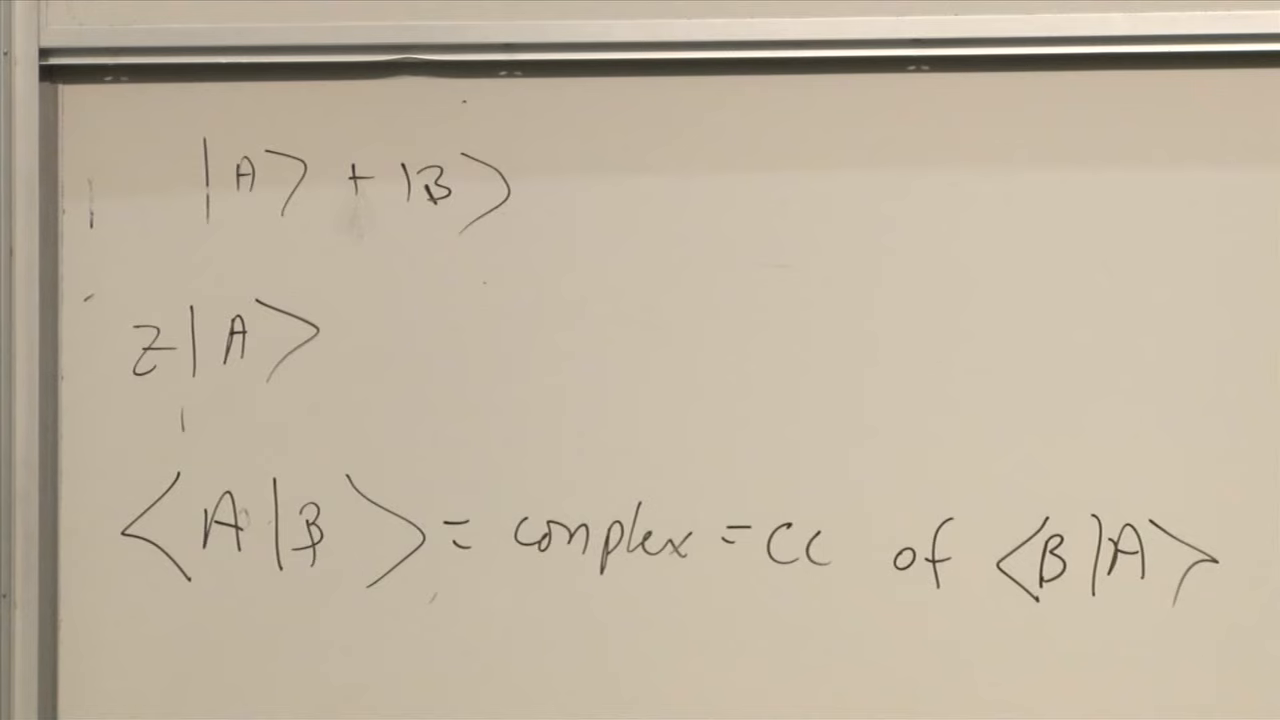
\includegraphics[width=0.78\textwidth]{lecture_02_figure_05.png}
\caption{この板書は線形結合と内積の共役反転を要約している。}
\lectureframe{00:46:53}
\end{figure}

ベクトルの長さの二乗は
\begin{equation}
\|\ket{A}\|^2=\braket{A}{A}.
\end{equation}
式~\eqref{eq:conjugate-symmetry}により、この数は自身の複素共役に等しくなり、したがって実数である。内積の公理により、この数は非負でもある。二つのベクトルが直交するのは
\begin{equation}
\braket{A}{B}=0.
\end{equation}
のときである。空間の次元とは、互いに直交する零でない方向として選び得る最大の個数である。

\begin{classroomqa}
\audiencequestion{すべての基底は互いに直交するベクトルから成らなければならないのか。}
\lecturerresponse{いいえ。基底は線形独立でありさえすればよく、空間を張りさえすればよい。直交基底は、係数と確率を容易に取り出せるため特に便利である。2次元では、2つの非平行なベクトルは、その内積がゼロでなくても基底を成し得る。}
\end{classroomqa}

\section{2次元スピン空間}

1つのスピンの状態空間は2次元複素ベクトル空間であると仮定される。
\begin{equation}
\mathcal H_{\mathrm{spin}}\cong\mathbb C^2.
\end{equation}
可能な状態ベクトルは連続的に無数に存在するが、それらすべてを表すには2つの独立な基底ベクトルがあればよい。

\(z\)方向の装置で準備された状態から始める。
\begin{align}
\ket{u}&\longleftrightarrow \sigma_z=+1,\\
\ket{d}&\longleftrightarrow \sigma_z=-1.
\end{align}
文字\(u,d\)、符号\(+,-\)、矢印\(\uparrow,\downarrow\)は、同じ2つの準備状態に対する別のラベルである。\(z\)測定はそれらを確実に区別するので、それらの状態ベクトルは直交する。
\begin{equation}
\braket{u}{d}=0.
\end{equation}
それらを単位長さに選ぶ。
\[
\braket{u}{u}=\braket{d}{d}=1.
\]

すると、すべてのスピン状態は次のように書ける。
\begin{equation}
\ket{A}=\alpha_u\ket{u}+\alpha_d\ket{d},
\qquad \alpha_u,\alpha_d\in\mathbb C.
\label{eq:general-spin-state}
\end{equation}
確率規則は次のとおりである。
\begin{equation}
P(u|A)=|\alpha_u|^2,\qquad
P(d|A)=|\alpha_d|^2.
\label{eq:born-z}
\end{equation}
2つの結果のうち一方が必ず起こるので、
\begin{equation}
|\alpha_u|^2+|\alpha_d|^2=1.
\label{eq:normalization}
\end{equation}

\begin{figure}[htbp]
\centering
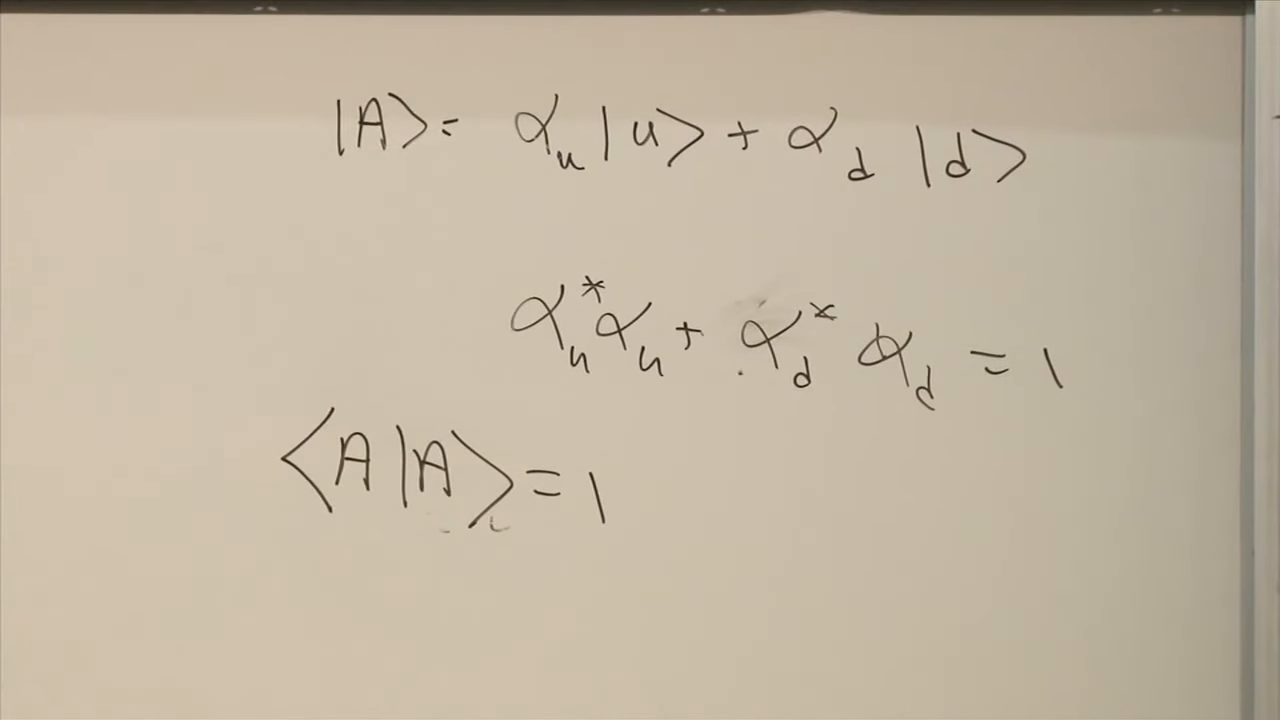
\includegraphics[width=0.78\textwidth]{lecture_02_figure_06.png}
\caption{一般的な上--下展開、2つの結果の確率の和、および等価な単位ノルム条件。}
\lectureframe{01:03:38}
\end{figure}

単位規格化との等価性は直接に導かれる。
\begin{align}
\braket{A}{A}
&=(\alpha_u^*\bra{u}+\alpha_d^*\bra{d})
  (\alpha_u\ket{u}+\alpha_d\ket{d})\\
&=|\alpha_u|^2\braket{u}{u}
 +\alpha_u^*\alpha_d\braket{u}{d}\\
&\quad +\alpha_d^*\alpha_u\braket{d}{u}
 +|\alpha_d|^2\braket{d}{d}\\
&=|\alpha_u|^2+|\alpha_d|^2=1.
\end{align}
したがって、物理的な純粋状態は規格化されたベクトルで表される。

\begin{classroomqa}
\audiencequestion{これらの記述は導出されているのか、それとも公理なのか。}
\lecturerresponse{現時点では、これらは実験に合わせて調整されている規則である。2次元空間、確率規則、および直交性の解釈は発見的に導入されている。それらの相互整合性は今すぐ確認できる。状態と観測量の体系的な関係は次に来る。}
\end{classroomqa}

\subsection{区別可能性としての直交性}

直交性の物理的内容は、垂直な矢印の描像よりも有用である。

\begin{quote}
1回の測定によって確実に区別できる状態は、直交するベクトルで表される。
\end{quote}

上と下はこの基準を満たす。状態が上であれば、\(z\)装置は決して下を報告せず、その逆も同様である。重なりがゼロでないことは、一方の状態が他方に関連する結果を時々生じ得ることを示す。

\section{右--左基底}

\(\ket{r}\)と\(\ket{l}\)を、\(x\)スピンの確定した状態を表すものとする。
\[
\ket{r}\longleftrightarrow\sigma_x=+1,\qquad
\ket{l}\longleftrightarrow\sigma_x=-1.
\]
空間は2次元であるから、それぞれは\(\ket{u}\)と\(\ket{d}\)の線形結合でなければならない。右に準備されたスピンは上と下を等しい確率で与えるので、2つの係数の大きさは等しくなければならない。最も単純な位相の規約を選ぶ。
\begin{equation}
\ket{r}=\frac{1}{\sqrt2}\bigl(\ket{u}+\ket{d}\bigr).
\label{eq:right-state}
\end{equation}
右と左は\(x\)装置によって確実に区別できるので、左状態は右状態に直交しなければならない。便利な選択の1つは次のとおりである。
\begin{equation}
\ket{l}=\frac{1}{\sqrt2}\bigl(\ket{u}-\ket{d}\bigr).
\label{eq:left-state}
\end{equation}
実際、
\begin{align}
\braket{l}{r}
&=\frac12(\bra{u}-\bra{d})(\ket{u}+\ket{d})\\
&=\frac12(1-1)=0.
\end{align}

\begin{figure}[htbp]
\centering
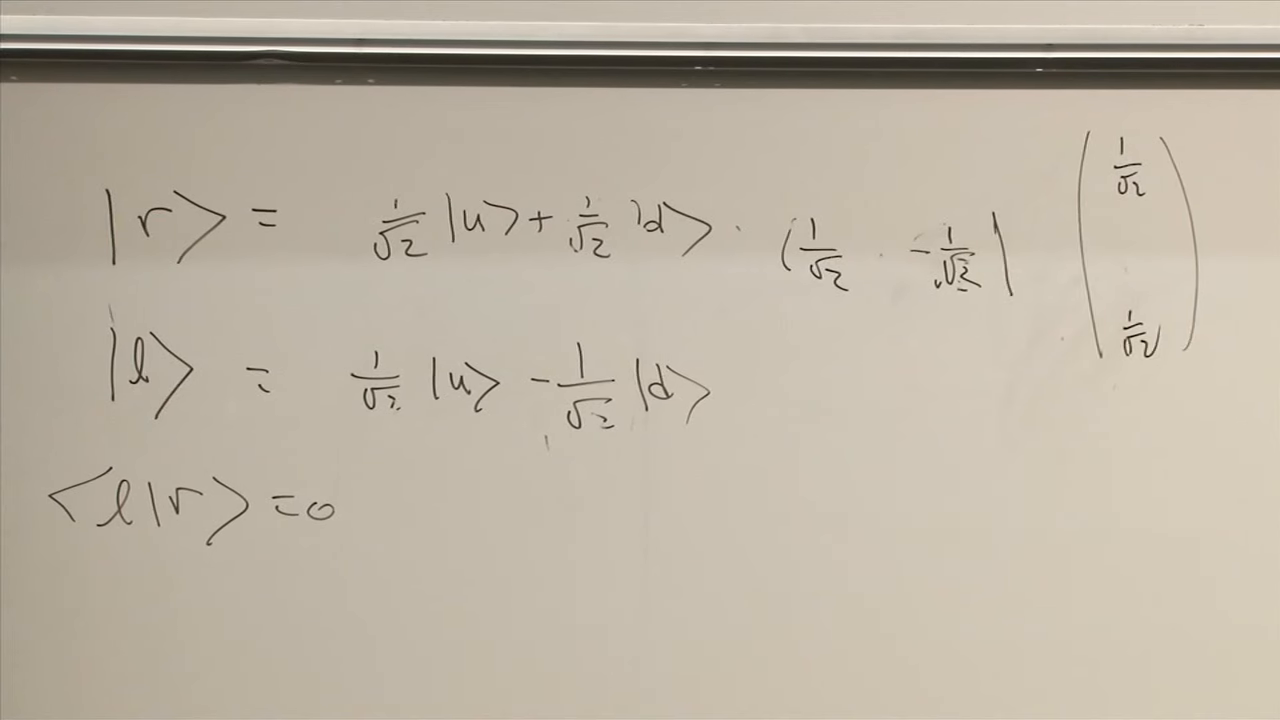
\includegraphics[width=0.82\textwidth]{lecture_02_figure_07.png}
\caption{完成した右--左の構成：上--下の大きさが等しく、相対符号が逆で、内積がゼロ。}
\lectureframe{01:12:15}
\end{figure}

\(\ket{l}\)の全体の負符号は規約である。\(\ket{l}\)を\(-\ket{l}\)に置き換えても、その確率は何も変わらない。式~\eqref{eq:right-state}と~\eqref{eq:left-state}を加減すると、逆の基底変換が得られる。
\begin{align}
\ket{u}&=\frac{1}{\sqrt2}\bigl(\ket{r}+\ket{l}\bigr),\\
\ket{d}&=\frac{1}{\sqrt2}\bigl(\ket{r}-\ket{l}\bigr).
\end{align}
この対称性は重要である。\(x\)基底から出発すると、上または下の状態は右と左の等重みの重ね合わせであり、ちょうど右または左の状態が上と下の等重みの重ね合わせであるのと同じである。

\section{入--出基底と相対位相}

装置を\(y\)に沿って、板に垂直に配向する。次のように書く。
\[
\ket{i}\longleftrightarrow\sigma_y=+1,\qquad
\ket{o}\longleftrightarrow\sigma_y=-1,
\]
ここでケットのラベル\(i\)は\emph{入}を意味し、ケットに掛かる装飾のない\(i\)は虚数単位のままである。

上と下の確率が等しいことは、係数の大きさが等しいことを要求する。入と出の間の直交性は、それらの重なりをゼロにする相対位相を要求する。対称的な選択は次のとおりである。
\begin{align}
\ket{i}&=\frac{1}{\sqrt2}\bigl(\ket{u}+i\ket{d}\bigr),\\
\ket{o}&=\frac{1}{\sqrt2}\bigl(\ket{u}-i\ket{d}\bigr).
\label{eq:in-out-states}
\end{align}
\((u,d)\)基底では、6つの状態はすべて次のようになる。
\begin{align}
\ket{u}&=\binom10,
&
\ket{d}&=\binom01,
\\
\ket{r}&=\frac1{\sqrt2}\binom11,
&
\ket{l}&=\frac1{\sqrt2}\binom1{-1},
\\
\ket{i}&=\frac1{\sqrt2}\binom1{i},
&
\ket{o}&=\frac1{\sqrt2}\binom1{-i}.
\end{align}

\begin{figure}[htbp]
\centering
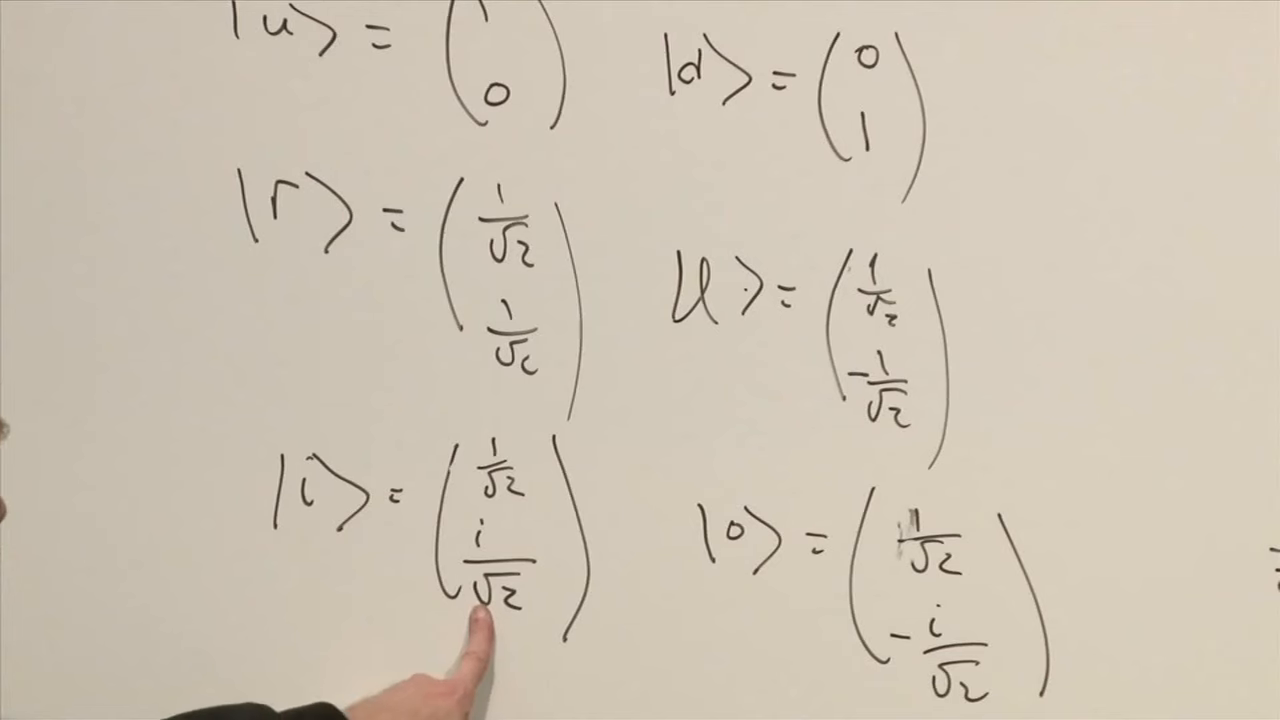
\includegraphics[width=0.82\textwidth]{lecture_02_figure_08.png}
\caption{上--下基底における6つの列ベクトル。下の対は相対的な虚数位相の符号だけが異なる。}
\lectureframe{01:20:50}
\end{figure}

直交性の確認には、ブラにおける複素共役が不可欠である。
\begin{align}
\braket{i}{o}
&=\frac12(\bra{u}-i\bra{d})(\ket{u}-i\ket{d})\\
&=\frac12\bigl(1+(-i)(-i)\bigr)=0.
\end{align}

\begin{classroomqa}
\audiencequestion{\emph{in}に対して\emph{out}ではなく\(+i\)を選ぶことは、空間軸の利き手性をエンコードしているのか？}
\lecturerresponse{一つの規約が導入された。その幾何学的意味は、パウリ行列と回転が展開されるときにより明確になるであろう。今のところ、この対は直交し、他の基底と対称的に関係していなければならない。ラベルを交換すること、あるいは\(y\)軸を反転することは、規約を変えるのであって、構成の整合性を変えるのではない。}
\end{classroomqa}

\subsection{右--左基底における対称性の確認}

イン状態において
\[
\ket{u}=\frac{\ket{r}+\ket{l}}{\sqrt2},\qquad
\ket{d}=\frac{\ket{r}-\ket{l}}{\sqrt2}
\]
を用いる：
\begin{align}
\ket{i}
&=\frac1{\sqrt2}
\left(
\frac{\ket{r}+\ket{l}}{\sqrt2}
+i\frac{\ket{r}-\ket{l}}{\sqrt2}
\right)\\
&=\frac{1+i}{2}\ket{r}
 +\frac{1-i}{2}\ket{l}.
\label{eq:in-in-rl}
\end{align}
どちらの係数にも\(1/\sqrt2\)が目に見える形では含まれていないが、
\begin{equation}
\left|\frac{1+i}{2}\right|^2
=\left|\frac{1-i}{2}\right|^2
=\frac12.
\end{equation}

\begin{figure}[htbp]
\centering
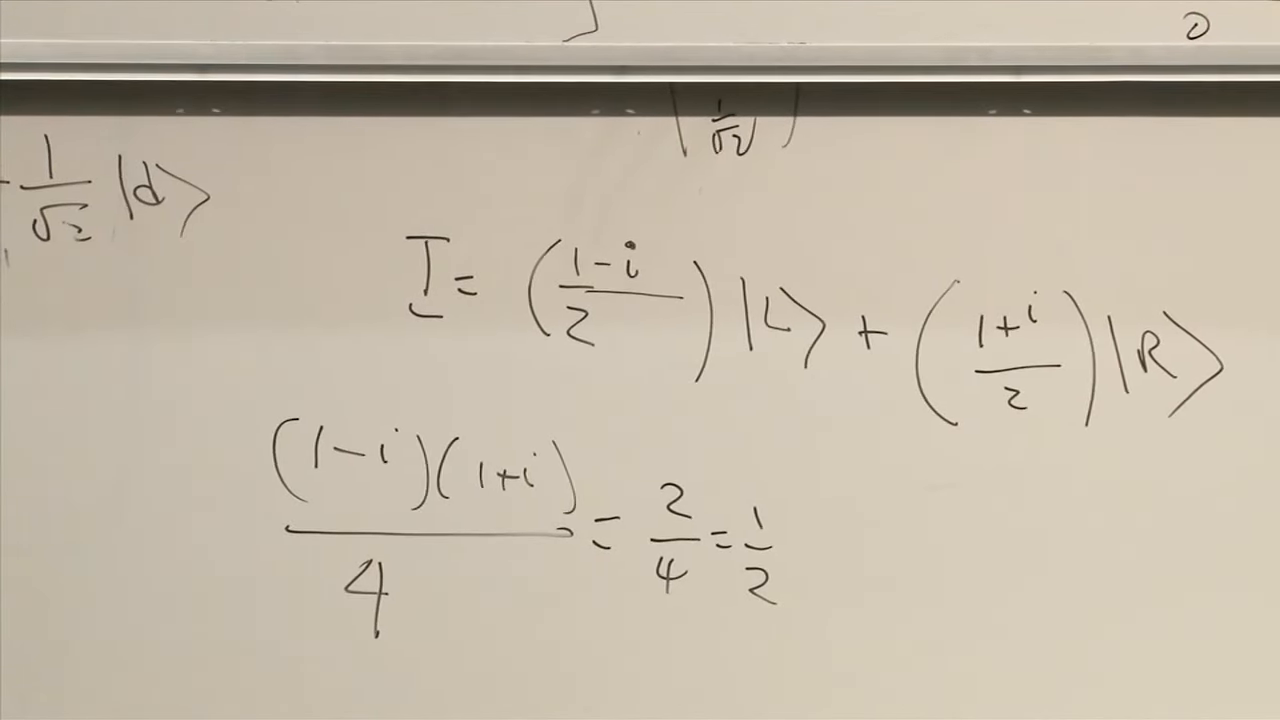
\includegraphics[width=0.82\textwidth]{lecture_02_figure_09.png}
\caption{イン状態に対する基底の実際の変更と、各右--左確率が\(1/2\)であることの確認。}
\lectureframe{01:29:10}
\end{figure}

したがって、三つの基底のうちの一つにおける各状態は、他の二つの基底のいずれかで測定されるときに等しい確率を与える。\(z\)、\(x\)、\(y\)基底は互いに不偏である。

\section{なぜ三つの特別な基底対が存在するのか}

\begin{classroomqa}
\audiencequestion{これら三つの対が互いに対してそうであるのと同じくらい対称的に関係する第四の状態対が存在しうるか？}
\lecturerresponse{単一の二状態系については存在しない。三つの互いに不偏な対が固定されると、同じ等しい重なり関係をもつ第四の対は存在しない。このような空間的ラベルが三つあるという事実は、複素状態空間自体の次元が二であるにもかかわらず、通常の空間の三次元と結びついている。}
\end{classroomqa}

この結びつきは物理的パラメータを数えることによって見ることができる。一般の列
\[
\binom{\alpha_u}{\alpha_d}
\]
は二つの複素数、したがって四つの実数を含む。規格化が一つを除く：
\[
|\alpha_u|^2+|\alpha_d|^2=1.
\]
両方の成分に共通の位相を掛けても測定確率は変わらない：
\begin{equation}
\ket{A}\sim e^{i\chi}\ket{A}.
\label{eq:global-phase}
\end{equation}
これがさらにもう一つの実パラメータを除く。したがって
\begin{equation}
4-1-1=2
\end{equation}
物理的実パラメータが残り、これは三次元空間における方向を指定するのに必要な角度の数とちょうど同じである。

便利な代表が関係を明示する：
\begin{equation}
\ket{\psi(\theta,\phi)}
=\cos\frac{\theta}{2}\,\ket{u}
+e^{i\phi}\sin\frac{\theta}{2}\,\ket{d}.
\label{eq:bloch-parameterization}
\end{equation}
\editorialnote{式~\eqref{eq:bloch-parameterization}は、講義で同定された二パラメータ族の標準的な規格化された代表である。明示的な半角の形はパラメータの数を具体的にするために含まれている。その力学的および回転的解釈は後の講義に属する。}

\begin{classroomqa}
\audiencequestion{全体位相を無視することの正確な数学は何か？}
\lecturerresponse{円\(\{e^{i\chi}\ket{\psi}\}\)上のすべての規格化されたベクトルは同じ物理的状態を表す。それらのベクトルを等価なものとして同一視する。ちょうど、宣言された冗長性によって関係づけられた点が一つの物理的点として扱われるのと同様である。成分間の相対位相は測定可能なままである。ベクトル全体に掛かる位相だけが捨てられる。}
\end{classroomqa}

\begin{classroomqa}
\audiencequestion{規格化されていないベクトルや負の成分をもつベクトルが計算に現れてもよいか？}
\lecturerresponse{よい。線形代数はそれらを許容し、中間的なベクトルはまだ準備された物理的状態を表す必要はない。非零ベクトルは最後に規格化できる。負および複素の成分は振幅であり、負の確率ではない。確率は状態が規格化された後に絶対値の二乗から生じる。}
\end{classroomqa}

\begin{classroomqa}
\audiencequestion{この描像はより高次元の空間、あるいはより複雑なスピノルに対してどうなるか？}
\lecturerresponse{同じ線形原理が続くが、状態空間の次元、空間的回転、観測可能なスピンの間の関係はより豊かになる。その拡張は現在の二状態構成の範囲外である。}
\end{classroomqa}

\section{直交性は空間的垂直性ではない}

\emph{直交}という語は今や抽象的で操作的な意味をもつ。通常の空間に描かれた二つの矢印の間の角度と混同してはならない。空間的方向の上と下は反対であるが、状態ベクトル\(\ket{u}\)と\(\ket{d}\)は直交している。空間的方向の上と右は垂直であるが、
\begin{equation}
\braket{u}{r}=\frac1{\sqrt2}\ne0.
\end{equation}

\begin{classroomqa}
\audiencequestion{反対の空間的方向が直交し、垂直な空間的方向が直交しないのはなぜか？}
\lecturerresponse{状態空間の重なりは実験的な識別可能性を測るのであって、ラベル間のユークリッド角を測るのではない。上と下は一回の\(z\)測定によって確実に区別できるので、それらの重なりは消える。上と右はそうではない。右に準備されたスピンは時に上の結果を与える。したがってそれらの状態ベクトルは重なる。}
\end{classroomqa}

同じ考え方には古典的な確率論における類似物がある。台が互いに素な二つの確率分布は完全に識別可能である。観測された結果はどちらの分布が用いられたかを特定する。台が重なり合う分布は、一つの標本からは誤りなく識別できない。量子力学的な直交性が非重複の役割を果たし、内積がゼロでないことは、ある結果がどちらの準備とも両立しうることを示す。

\begin{classroomqa}
\audiencequestion{二次元の状態空間は、上向きと右向きの矢印を含む物理的な平面として思い描くべきだろうか。}
\lecturerresponse{そうではない。ラベル\(x,y,z\)は通常の空間における装置の向きを指す。ケットはそれ自身の内積をもつ複素ベクトル空間に属する。パラメータの数が二つの構造を結びつけるが、それらの描像を点ごとに同一視すると、空間的な垂直性と状態空間の直交性を混同することになる。}
\end{classroomqa}

\section{状態、測定、そしてこれからなすべきこと}

これまでの構成は、ベクトルを操作的な事実に当てはめることによって進められてきた。三つの装置の向きは三対の規格化された状態にラベルを付け、その重なりが観測された確率を再現する。厳密な取り扱いでは、\(\sigma_z\)のような可観測量が状態にどのように作用するのか、そしてなぜその可能な結果がその固有値であるのかを、なお述べなければならない。それが次の段階である。

先ほどの論理的なパズルは、今やより鋭く述べることができる。命題は部分空間またはその射影演算子に対応し、両立しない射影演算子は可換でない。順序に敏感なORのテストは言葉の上の逆説ではなく、この非可換構造の初期の現れであった。

\begin{classroomqa}
\audiencequestion{状態が通常の矢印でないのなら、なぜ三つのラベル\(x,y,z\)と平均\(\langle\sigma_{\hat m}\rangle\)はこれほど古典的に見えるのか。}
\lecturerresponse{古典的なベクトルはアンサンブル平均に現れる。単一のスピンは離散的な答えを与えるが、同じように準備された多数のスピンは、ある方向の成分のように変換する平均を与える。巨視的な古典的振る舞いは、大きな集団がそれらの平均を安定させることによって現れる。それを、個々のスピンの中に隠れた連続的な値があると逆に読み取るべきではない。}
\end{classroomqa}

\begin{classroomqa}
\audiencequestion{共通位相の冗長性はゲージ不変性の一例だろうか。}
\lecturerresponse{それは共通位相の下での単純な不変性であり、より広いゲージの考え方を予示している。ここでそのつながりを展開するのは現在の構成の範囲を超えるので、物理的に関連する主張だけを保持する。すなわち、共通位相は見えず、相対位相は見えないわけではない。}
\end{classroomqa}

最後に、測定は、スピンが古典的な意味でずっと前から担っていた値を単に明るみに出すものとして思い描くべきではない。測定は、記録された結果に対応する状態を準備する。したがって、同じ測定を直ちに繰り返すことは整合的であり、一方、同じように準備されたスピンの新しいアンサンブルは、対応する振幅によって定まる確率分布を示す。その準備と読み出しの数学的記述は、可観測量が演算子として導入されれば正確になる。